% Options for packages loaded elsewhere
\PassOptionsToPackage{unicode}{hyperref}
\PassOptionsToPackage{hyphens}{url}
%
\documentclass[
]{book}
\usepackage{lmodern}
\usepackage{amssymb,amsmath}
\usepackage{ifxetex,ifluatex}
\ifnum 0\ifxetex 1\fi\ifluatex 1\fi=0 % if pdftex
  \usepackage[T1]{fontenc}
  \usepackage[utf8]{inputenc}
  \usepackage{textcomp} % provide euro and other symbols
\else % if luatex or xetex
  \usepackage{unicode-math}
  \defaultfontfeatures{Scale=MatchLowercase}
  \defaultfontfeatures[\rmfamily]{Ligatures=TeX,Scale=1}
\fi
% Use upquote if available, for straight quotes in verbatim environments
\IfFileExists{upquote.sty}{\usepackage{upquote}}{}
\IfFileExists{microtype.sty}{% use microtype if available
  \usepackage[]{microtype}
  \UseMicrotypeSet[protrusion]{basicmath} % disable protrusion for tt fonts
}{}
\makeatletter
\@ifundefined{KOMAClassName}{% if non-KOMA class
  \IfFileExists{parskip.sty}{%
    \usepackage{parskip}
  }{% else
    \setlength{\parindent}{0pt}
    \setlength{\parskip}{6pt plus 2pt minus 1pt}}
}{% if KOMA class
  \KOMAoptions{parskip=half}}
\makeatother
\usepackage{xcolor}
\IfFileExists{xurl.sty}{\usepackage{xurl}}{} % add URL line breaks if available
\IfFileExists{bookmark.sty}{\usepackage{bookmark}}{\usepackage{hyperref}}
\hypersetup{
  pdftitle={Knowledge Pool},
  pdfauthor={Martyna Bogacz},
  hidelinks,
  pdfcreator={LaTeX via pandoc}}
\urlstyle{same} % disable monospaced font for URLs
\usepackage{longtable,booktabs}
% Correct order of tables after \paragraph or \subparagraph
\usepackage{etoolbox}
\makeatletter
\patchcmd\longtable{\par}{\if@noskipsec\mbox{}\fi\par}{}{}
\makeatother
% Allow footnotes in longtable head/foot
\IfFileExists{footnotehyper.sty}{\usepackage{footnotehyper}}{\usepackage{footnote}}
\makesavenoteenv{longtable}
\usepackage{graphicx,grffile}
\makeatletter
\def\maxwidth{\ifdim\Gin@nat@width>\linewidth\linewidth\else\Gin@nat@width\fi}
\def\maxheight{\ifdim\Gin@nat@height>\textheight\textheight\else\Gin@nat@height\fi}
\makeatother
% Scale images if necessary, so that they will not overflow the page
% margins by default, and it is still possible to overwrite the defaults
% using explicit options in \includegraphics[width, height, ...]{}
\setkeys{Gin}{width=\maxwidth,height=\maxheight,keepaspectratio}
% Set default figure placement to htbp
\makeatletter
\def\fps@figure{htbp}
\makeatother
\setlength{\emergencystretch}{3em} % prevent overfull lines
\providecommand{\tightlist}{%
  \setlength{\itemsep}{0pt}\setlength{\parskip}{0pt}}
\setcounter{secnumdepth}{5}
\usepackage{booktabs}
\usepackage{amsthm}
\makeatletter
\def\thm@space@setup{%
  \thm@preskip=8pt plus 2pt minus 4pt
  \thm@postskip=\thm@preskip
}
\makeatother
\usepackage[]{natbib}
\bibliographystyle{apalike}

\title{Knowledge Pool}
\author{Martyna Bogacz}
\date{2021-01-15}

\begin{document}
\maketitle

{
\setcounter{tocdepth}{1}
\tableofcontents
}
\hypertarget{preface}{%
\chapter*{Preface}\label{preface}}
\addcontentsline{toc}{chapter}{Preface}

\begin{enumerate}
\def\labelenumi{\arabic{enumi}.}
\tightlist
\item
  Introduction to the knowledge pool \ref{intro}
\item
  Physical road infrastructure \ref{infrastructure}
\item
  Highway infrastructure management \ref{highway}
\item
  Traffic management \ref{traffic}
\item
  Road pricing \ref{pricing}
\item
  Digital road infrastructure and connectivity \ref{digital}
\item
  Passenger information system \ref{passenger}
\item
  Multimodal integrated system \ref{multimodal}
\item
  Connected and autonomous driving \ref{connected}
\item
  On-board technology for connected and automated vehicles \ref{onboard}
\item
  Freight and commercial transport \ref{freight}
\item
  Collective mobility vehicles \ref{collective}
\item
  Big data \ref{big}
\item
  Shared mobility \ref{shared}
\item
  Alternative power sources \ref{alternative}
\end{enumerate}

\hypertarget{intro}{%
\chapter{Introduction}\label{intro}}

This work gathers and defines essential concepts related to automation and digitalisation of transport system together with the description of their impact, both negative and positive on \textbf{individual}, \textbf{systemic} and \textbf{economy level}. This knowledge pool is driven by the fact that automation and digitalisation are progressing quickly, although not uniformly across all areas within transport context. Therefore, to understand spectrum of possibilities that they bring, it is necessary to explain key concepts, demonstrate their level of maturity and current market penetration, and finally assess their impact on different levels. Given this approach, the page of each topic contains the following elements:\textbf{definition} of the phenomenon,
\textbf{key stakeholders} who are the main parties responsible for and affected by the given technological development. Then, we include two subsections on \textbf{current state of art in research and practice}. The former one summarizes the most recent research in a given topic while the latter explains the current stage of implementation of given technology in the real world. Further, section named \textbf{relevant initatives in Austria} covers the leading initaitives within given topic and potential for Austrain actors. Moreover, we provide the summary table of the impacts of the concept on selected \textbf{sustainable development goals} (SDGs). Beyond, to provide an objective measure of technology maturity within each topic we include so-called \textbf{technology readiness scale} (Willismson \& Beasley, 2011) and \textbf{societal readiness scale}, as described below:

\begin{figure}
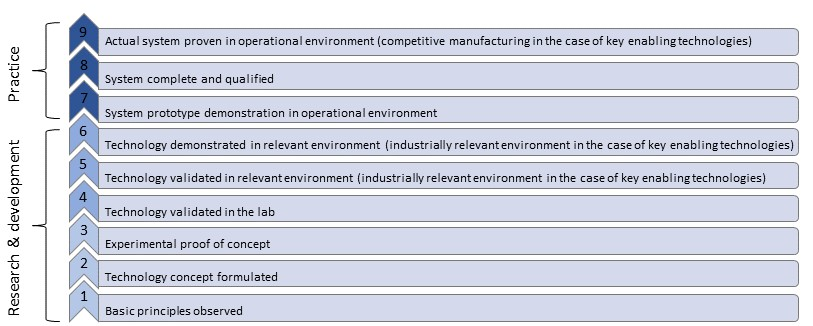
\includegraphics[width=2\linewidth]{image/TRL} \caption{Technology readiness scale}\label{fig:unnamed-chunk-1}
\end{figure}

\begin{figure}
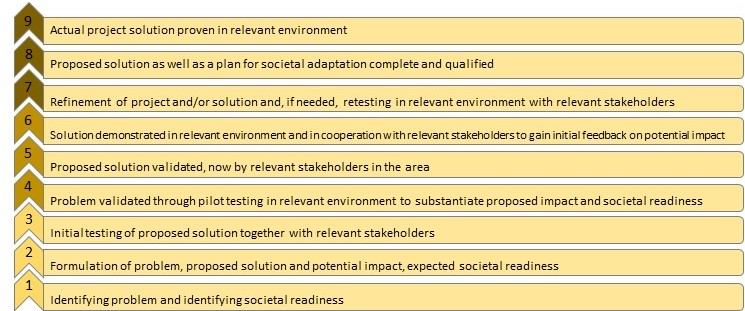
\includegraphics[width=2\linewidth]{image/SRL} \caption{Societal readiness scale}\label{fig:unnamed-chunk-2}
\end{figure}

Finally, we provide a list of \textbf{outstanding questions} and \textbf{links to additional sources} on the topic.

\textbf{References}

\begin{itemize}
\tightlist
\item
  Williamson, R., \& Beasley, J. (2011). Automotive technology and manufacturing readiness levels: a guide to recognised stages of development within the automotive industry. URN11/672.
\end{itemize}

\hypertarget{infrastructure}{%
\chapter{Physical road infrastructure}\label{infrastructure}}

\hypertarget{dedicated-lanes-for-connected-and-automated-vehicles-cav}{%
\section{Dedicated lanes for connected and automated vehicles (CAV)}\label{dedicated-lanes-for-connected-and-automated-vehicles-cav}}

\hypertarget{synonyms}{%
\subsection{Synonyms}\label{synonyms}}

\emph{AV-dedicated lanes}, \emph{dedicated corridors}

\hypertarget{definition}{%
\subsection{Definition}\label{definition}}

Dedicated lane for connected and autonomous vehicles features additional infrastructure or sensors to increase the reliability of Advanced Driver Assistant Systems (ADAS). Only automated driving vehicles are allowed to drive on these lanes. The typical applications include cooperative and adaptive cruise control based on sensors with the infrastructure, lane keeping, fuel use optimization and road pricing possibilities (Broek et al., 2011). The introduction of dedicated lanes for CAV is expected to have direct consequences on the traffic flow on the highways and a nearby road network. In particular, a study conducted in Singapore showed that dedicated lanes on the highways can reduce travel time of CAVs by approximately 25\% (if the saturation on the lane is not reached) at the cost of a delay for conventional cars of approximately 7\%, due to the reduced capacity (Ivanchev et al., 2017). They were also demonstrated to have a positive effect on fuel consumption.
Moreover, the throughput, defined as a number of vehicles passing through the road in a given time interval, increased as a result of introduction of dedicated lanes for AVs (Kumar et al., 2020). This effect, however, was associated with a decrease in throughput of smaller roads due to the preference of AVs for highways because of time savings, which in turn can result in time loss for conventional cars. What is more, the benefits from increased capacity of AV-only lanes can be further amplified through setting a higher speed limits for these lanes (Ye \& Yamamoto, 2018). With respect to the demand for different road types the study found that the introduction of dedicated CAV lanes will increase the demand of conventional cars for major road (but smaller than highways) and minor roads as a substitution for more congested highways due to the dedicated AV lanes.
In contrast, study by Chen et al.~(2016) showed that the implementation of CAV dedicated lanes has a potential of maximizing traffic capacity on these lanes in a mix-traffic context while having effectively no impact on conventional traffic capacity. Further, in order to use efficiently CAV dedicated lanes, which may be underutilized at the early stage, it is proposed to allow conventional cars to enter the AVs-only lanes after toll payment. This solution stems from currently operational across the world High Occupancy Vehicle (HOV) lanes. This joint approach is claimed to improve the throughput of individual road as well as enhance system-wide flow distribution within the network (Liu \& Song, 2019).

\hypertarget{key-stakeholders}{%
\subsection{Key stakeholders}\label{key-stakeholders}}

\begin{itemize}
\tightlist
\item
  \textbf{Affected}: Conventional Cars' Drivers, Car Manufacturers, Insurers
\item
  \textbf{Responsible}: Road Infrastructure Agencies, Local and National Governments
\end{itemize}

\hypertarget{current-state-of-art-in-research}{%
\subsection{Current state of art in research}\label{current-state-of-art-in-research}}

Current research focuses on gathering the evidence of the impact of the introduction of dedicated lanes on traffic flow, driver behavior adoption, safety and efficiency. Furthermore, it analyses the factors which influence them, by testing different design and operation configurations, road types and utilization policies (Rad et al., 2020). Both, field operational testing and driving simulator studies have been conducted to investigate the influence of different designs of dedicated lanes on drivers in conventional cars and those featuring some degree of automation (Guin et al., 2008, Zhong, 2018). In particular, a number of studies compared distinct access types of dedicated lanes (Zhong, 2018, Yang et al., 2019). They showed that dedicated lanes with limited access performed better in terms of travel time and throughput compared to dedicated lanes with continuous access. Moreover, the probability of vehicles platooning was significantly higher on dedicated lanes with limited access. On the other hand, it was showed that collision rates near the entry or exit of these limited access lanes are higher (Rad et al.~2020).

\hypertarget{current-state-of-art-in-practice}{%
\subsection{Current state of art in practice}\label{current-state-of-art-in-practice}}

Currently state of Michigan together with several private partners including Ford and Alphabet Inc.~are planning to dedicate 65 km of a highway between Detroit and Ann Arbor for the sole movement of autonomous vehicles including buses and shuttles (Krisher \& Eggert, 2020). Similar initiatives are taking place in other countries, for instance, China set out to build nearly 100 km of 8-lane highway linking Beijing and the Xiongan New Area, from which 2 lanes will be allocated for the automated traffic. The completion of the construction phase is predicted by the end of 2020, while its opening is for traffic is expected in June 2021 (Syncedreview.com, 2020). In Europe, there is on-going SHOW (SHared automation Operating models for Worldwide adoption) project which aims to deploy about seventy automated vehicles in 21 European cities. To assess how they can best be integrated vehicles will be used in different settings in mixed traffic and dedicated lanes. However, for safety reasons the driver will be on-board (CORDIS, 2020).

\hypertarget{relevant-initiatives-in-austria}{%
\subsection{Relevant initiatives in Austria}\label{relevant-initiatives-in-austria}}

\begin{itemize}
\tightlist
\item
  \href{https://www.tugraz.at/fileadmin/user_upload/Institute/IHF/Projekte/ENABLE-S3_SummaryofResults_May2019.pdf}{tugraz.at}
\item
  \href{https://www.ait.ac.at/themen/verkehrssicherheit-und-unfallforschung/projects/via-autonom/}{ait.ac.at}
\end{itemize}

\hypertarget{impacts-with-respect-to-sustainable-development-goals-sdgs}{%
\subsection{Impacts with respect to Sustainable Development Goals (SDGs)}\label{impacts-with-respect-to-sustainable-development-goals-sdgs}}

\begin{longtable}[]{@{}ccccc@{}}
\toprule
\begin{minipage}[b]{0.17\columnwidth}\centering
Impact level\strut
\end{minipage} & \begin{minipage}[b]{0.16\columnwidth}\centering
Indicator\strut
\end{minipage} & \begin{minipage}[b]{0.17\columnwidth}\centering
Impact direction\strut
\end{minipage} & \begin{minipage}[b]{0.17\columnwidth}\centering
Goal description and number\strut
\end{minipage} & \begin{minipage}[b]{0.17\columnwidth}\centering
Source\strut
\end{minipage}\tabularnewline
\midrule
\endhead
\begin{minipage}[t]{0.17\columnwidth}\centering
Individual\strut
\end{minipage} & \begin{minipage}[t]{0.16\columnwidth}\centering
Fuel consumption reduced\strut
\end{minipage} & \begin{minipage}[t]{0.17\columnwidth}\centering
+\strut
\end{minipage} & \begin{minipage}[t]{0.17\columnwidth}\centering
Environmental sustainability (\emph{7,12-13,15})\strut
\end{minipage} & \begin{minipage}[t]{0.17\columnwidth}\centering
Ivanchev et al., 2017\strut
\end{minipage}\tabularnewline
\begin{minipage}[t]{0.17\columnwidth}\centering
Individual\strut
\end{minipage} & \begin{minipage}[t]{0.16\columnwidth}\centering
Travel time reduced\strut
\end{minipage} & \begin{minipage}[t]{0.17\columnwidth}\centering
+\strut
\end{minipage} & \begin{minipage}[t]{0.17\columnwidth}\centering
Sustainable economic development (\emph{8,11})\strut
\end{minipage} & \begin{minipage}[t]{0.17\columnwidth}\centering
Zhong, 2018;Yang et al., 2019\strut
\end{minipage}\tabularnewline
\begin{minipage}[t]{0.17\columnwidth}\centering
Systemic\strut
\end{minipage} & \begin{minipage}[t]{0.16\columnwidth}\centering
Collision rate reduced\strut
\end{minipage} & \begin{minipage}[t]{0.17\columnwidth}\centering
+\strut
\end{minipage} & \begin{minipage}[t]{0.17\columnwidth}\centering
Health \& Wellbeing (\emph{3})\strut
\end{minipage} & \begin{minipage}[t]{0.17\columnwidth}\centering
Zhang et al., 2020\strut
\end{minipage}\tabularnewline
\begin{minipage}[t]{0.17\columnwidth}\centering
Systemic\strut
\end{minipage} & \begin{minipage}[t]{0.16\columnwidth}\centering
Emissions rate reduced\strut
\end{minipage} & \begin{minipage}[t]{0.17\columnwidth}\centering
+\strut
\end{minipage} & \begin{minipage}[t]{0.17\columnwidth}\centering
Environmental sustainability (\emph{7,12-13,15})\strut
\end{minipage} & \begin{minipage}[t]{0.17\columnwidth}\centering
Al Alam at al., 2010\strut
\end{minipage}\tabularnewline
\begin{minipage}[t]{0.17\columnwidth}\centering
Systemic\strut
\end{minipage} & \begin{minipage}[t]{0.16\columnwidth}\centering
Congestion\strut
\end{minipage} & \begin{minipage}[t]{0.17\columnwidth}\centering
\textasciitilde{}\strut
\end{minipage} & \begin{minipage}[t]{0.17\columnwidth}\centering
Sustainable economic development (\emph{8,11})\strut
\end{minipage} & \begin{minipage}[t]{0.17\columnwidth}\centering
Ivanchev et al., 2017;Kumar et al., 2020\strut
\end{minipage}\tabularnewline
\begin{minipage}[t]{0.17\columnwidth}\centering
Systemic\strut
\end{minipage} & \begin{minipage}[t]{0.16\columnwidth}\centering
Novel designs tested\strut
\end{minipage} & \begin{minipage}[t]{0.17\columnwidth}\centering
+\strut
\end{minipage} & \begin{minipage}[t]{0.17\columnwidth}\centering
Innovation \& Infrastructure (\emph{9})\strut
\end{minipage} & \begin{minipage}[t]{0.17\columnwidth}\centering
Guin et al., 2008;Zhong, 2018;Krisher \& Eggert, 2020\strut
\end{minipage}\tabularnewline
\begin{minipage}[t]{0.17\columnwidth}\centering
Systemic\strut
\end{minipage} & \begin{minipage}[t]{0.16\columnwidth}\centering
SHOW EU initiative\strut
\end{minipage} & \begin{minipage}[t]{0.17\columnwidth}\centering
+\strut
\end{minipage} & \begin{minipage}[t]{0.17\columnwidth}\centering
Partnership \& collaborations (\emph{17})\strut
\end{minipage} & \begin{minipage}[t]{0.17\columnwidth}\centering
CORDIS, 2020\strut
\end{minipage}\tabularnewline
\bottomrule
\end{longtable}

\hypertarget{technology-readiness-level}{%
\subsection{Technology readiness level}\label{technology-readiness-level}}

5-6

\hypertarget{societal-readiness-level}{%
\subsection{Societal readiness level}\label{societal-readiness-level}}

TBD

\hypertarget{open-questions}{%
\subsection{Open questions}\label{open-questions}}

\begin{enumerate}
\def\labelenumi{\arabic{enumi}.}
\tightlist
\item
  What are the potential benefits of dedicated AV lanes when coupled with smart platooning strategies?
\item
  How and to what degree will joint concepts by automotive sector, fleet and road
  operators will improve traffic management establishing dynamic traffic regulations even across
  borders?
\item
  What are the roles and responsibilities of the different stakeholders of physical infrastructure for connected and automated vehicles?
\item
  Should the vehicle cope with any road infrastructure, and if not, what demands can be set to adapt the existing infrastructure?
\item
  How to ensure continuity between those different environments?
\item
  Which tools (e.g.~micro- and macroscopic transport modelling, impact assessment) can enable
  cities to assess the impact of automated vehicles on their physical road infrastructure and
  balance the needs of automated vehicles against the needs of existing modes (conventional
  vehicles, public transport, pedestrians and cyclists). (ERTRAC, 2019)
\end{enumerate}

\hypertarget{further-links}{%
\subsection{Further links}\label{further-links}}

\begin{itemize}
\tightlist
\item
  \href{https://knowledge-base.connectedautomateddriving.eu/wp-content/uploads/2019/12/SMART_2010-0064-study-report-final_V1-2.pdf}{knowledge base}
\item
  \href{https://show-project.eu/}{show project}
\end{itemize}

\hypertarget{references}{%
\subsection{References}\label{references}}

\begin{itemize}
\tightlist
\item
  Al Alam, A., Gattami, A., \& Johansson, K. H. (2010, September). An experimental study on the fuel reduction potential of heavy duty vehicle platooning. In 13th International IEEE Conference on Intelligent Transportation Systems (pp.~306-311). IEEE.
  Broek, S. M., van Nunen, E., \& Zwijnenberg, H. (2011). Definition of necessary vehicle and infrastructure systems for automated driving. Retrieved January, 3, 2017.
\item
  Chen, Z., He, F., Zhang, L., \& Yin, Y. (2016). Optimal deployment of autonomous vehicle lanes with endogenous market penetration. Transportation Research Part C: Emerging Technologies, 72, 143-156.
\item
  CORDIS \textbar{} European Commission. (20 Apr 2020). Retrieved 13 November 2020, from \url{https://cordis.europa.eu/project/id/875530}
\item
  ERTRAC Working Group. (2019). Connected Automated Driving Roadmap. version, 8, 2019-08.
\item
  Guin, A., Hunter, M., \& Guensler, R. (2008). Analysis of reduction in effective capacities of high-occupancy vehicle lanes related to traffic behavior. Transportation Research Record, 2065(1), 47-53.
\item
  Ivanchev, J., Knoll, A., Zehe, D., Nair, S., \& Eckhoff, D. (2017). Potentials and implications of dedicated highway lanes for autonomous vehicles. arXiv preprint arXiv:1709.07658.
\item
  Krisher, T., \& Eggert, D. (14 Aug 2020). Michigan plans dedicated road lanes for autonomous vehicles. Retrieved 12 November 2020, from \url{https://abcnews.go.com/Technology/wireStory/michigan-plans-dedicated-road-lanes-autonomous-vehicles-72352758}
\item
  Kumar, A., Guhathakurta, S., \& Venkatachalam, S. (2020). When and where should there be dedicated lanes under mixed traffic of automated and human-driven vehicles for system-level benefits?. Research in Transportation Business \& Management, 100527.
\item
  Liu, Z., \& Song, Z. (2019). Strategic planning of dedicated autonomous vehicle lanes and autonomous vehicle/toll lanes in transportation networks. Transportation Research Part C: Emerging Technologies, 106, 381-403.
\item
  Rad, S. R., Farah, H., Taale, H., van Arem, B., \& Hoogendoorn, S. P. (2020). Design and operation of dedicated lanes for connected and automated vehicles on motorways: A conceptual framework and research agenda. Transportation Research Part C: Emerging Technologies, 117, 102664.
\item
  Syncedreview.com (31 Aug 2020). Beijing Builds 100km Highway Lanes for Self-Driving Cars with Unmanned Machineries. Retrieved 12 November 2020, from \url{https://syncedreview.com/2020/08/31/beijing-builds-100km-highway-lanes-for-self-driving-cars-with-unmanned-machineries/}
\item
  Yang, D., Farah, H., Schoenmakers, M. J., \& Alkim, T. (2019). Human drivers behavioural adaptation when driving next to a platoon of automated vehicles on a dedicated lane and implications on traffic flow: a driving simulator and microscopic simulation study in the Netherlands. In 98th Annual Meeting of the Transportation Research Board (pp.~19-00582).
\item
  Ye, L., \& Yamamoto, T. (2018). Impact of dedicated lanes for connected and autonomous vehicle on traffic flow throughput. Physica A: Statistical Mechanics and its Applications, 512, 588-597.
\item
  Zhang, J., Wu, K., Cheng, M., Yang, M., Cheng, Y., \& Li, S. (2020). Safety Evaluation for Connected and Autonomous Vehicles' Exclusive Lanes considering Penetrate Ratios and Impact of Trucks Using Surrogate Safety Measures. Journal of advanced transportation, 2020.
\item
  Zhong, Z. (2018). Assessing the effectiveness of managed lane strategies for the rapid deployment of cooperative adaptive cruise control technology.
\end{itemize}

\hypertarget{highway}{%
\chapter{Highway infrastructure management}\label{highway}}

\hypertarget{traffic}{%
\chapter{Traffic management}\label{traffic}}

\hypertarget{pricing}{%
\chapter{Road pricing}\label{pricing}}

\hypertarget{digital}{%
\chapter{Digital road infrastructure and connectivity}\label{digital}}

\hypertarget{passenger}{%
\chapter{Passenger information system}\label{passenger}}

\hypertarget{multimodal}{%
\chapter{Multimodal integrated system}\label{multimodal}}

\hypertarget{connected}{%
\chapter{Connected and autonomous driving}\label{connected}}

\hypertarget{onboard}{%
\chapter{On-board technology for connected and automated vehicles}\label{onboard}}

\hypertarget{freight}{%
\chapter{Freight and commercial transport}\label{freight}}

\hypertarget{collective}{%
\chapter{Collective mobility vehicles}\label{collective}}

\hypertarget{big}{%
\chapter{Big data}\label{big}}

\hypertarget{shared}{%
\chapter{Shared mobility}\label{shared}}

\hypertarget{alternative}{%
\chapter{Alternative power sources}\label{alternative}}

\hypertarget{reference}{%
\chapter{References}\label{reference}}

  \bibliography{book.bib,packages.bib}

\end{document}
